\documentclass[11pt]{beamer}
%\usepackage{CJKutf8}
\usepackage{beamerthemesplit}
\usepackage{}
%\usetheme{Frankfurt}
%\usetheme{CambridgeUS}
%\usecolortheme{beaver}
%\usetheme{AnnArbor}
\usetheme{Dresden}
%\usebeamercolor{beetle}
\usepackage{xeCJK}
\setCJKmainfont{AR PL KaitiM GB}
%\useoutertheme{miniframes}
\usepackage{amsmath}
\usepackage{graphicx}
\usepackage{float} 
\usepackage{subfigure}
\usepackage{amssymb}
\usepackage{graphicx}
\usepackage{eufrak}
\usepackage{color}
\usepackage{array}
\usepackage{slashed}
\usepackage{simplewick}
\usepackage{tikz}
\usepackage{tcolorbox}
\usepackage[T1]{fontenc}
\graphicspath{{../figures/}}

%%figures
\def\lfig#1#2{\includegraphics[width=#1 in]{#2}}
\def\addfig#1#2{\begin{center}\includegraphics[width=#1 in]{#2}\end{center}}
\def\wulian{
\includegraphics[width=0.18in]{emoji_wulian.jpg}}
\def\bigwulian{
\includegraphics[width=0.35in]{emoji_wulian.jpg}}
\def\bye{
\includegraphics[width=0.18in]{emoji_bye.jpg}}
\def\bigbye{
\includegraphics[width=0.35in]{emoji_bye.jpg}}
\def\huaixiao{
\includegraphics[width=0.18in]{emoji_huaixiao.jpg}}
\def\bighuaixiao{
\includegraphics[width=0.35in]{emoji_huaixiao.jpg}}
\def\jianxiao{
\includegraphics[width=0.18in]{emoji_jianxiao.jpg}}
\def\bigjianxiao{
\includegraphics[width=0.35in]{emoji_jianxiao.jpg}}
%% colors
\def\blacktext#1{{\color{black}#1}}
\def\bluetext#1{{\color{blue}#1}}
\def\redtext#1{{\color{red}#1}}
\def\darkbluetext#1{{\color[rgb]{0,0.2,0.6}#1}}
\def\skybluetext#1{{\color[rgb]{0.2,0.7,1.}#1}}
\def\cyantext#1{{\color[rgb]{0.,0.5,0.5}#1}}
\def\greentext#1{{\color[rgb]{0,0.7,0.1}#1}}
\def\darkgray{\color[rgb]{0.2,0.2,0.2}}
\def\lightgray{\color[rgb]{0.6,0.6,0.6}}
\def\gray{\color[rgb]{0.4,0.4,0.4}}
\def\blue{\color{blue}}
\def\red{\color{red}}
\def\green{\color{green}}
\def\darkgreen{\color[rgb]{0,0.4,0.1}}
\def\darkblue{\color[rgb]{0,0.2,0.6}}
\def\skyblue{\color[rgb]{0.2,0.7,1.}}
%%control
\def\be{\begin{equation}}
\def\ee{\nonumber\end{equation}}
\def\bea{\begin{eqnarray*}}
\def\eea{\nonumber\end{eqnarray*}}
\def\bch{}
\def\ech{}
\def\bitem{\begin{itemize}}
\def\eitem{\end{itemize}}
\def\bcenter{\begin{center}}
\def\ecenter{\end{center}}
\def\bex{\begin{minipage}{0.2\textwidth}
\includegraphics[width=0.6in]{jugelizi.png}\end{minipage}\begin{minipage}{0.76\textwidth}}
\def\eex{\end{minipage}}
\def\chtitle#1{\frametitle{\bch#1\ech}}
\def\bmat#1{\left(\begin{array}{#1}}
\def\emat{\end{array}\right)}
\def\bcase#1{\left\{\begin{array}{#1}}
\def\ecase{\end{array}\right.}
\def\bmini#1{\begin{minipage}{#1\textwidth}}
\def\emini{\end{minipage}}
\def\tbox#1{\begin{tcolorbox}#1\end{tcolorbox}}
\def\pfrac#1#2#3{\left(\frac{\partial #1}{\partial #2}\right)_{#3}}
%%symbols
\def\bropt{\,(\ \ \ )}
\def\sone{$\star$}
\def\stwo{$\star\star$}
\def\sthree{$\star\star\star$}
\def\sfour{$\star\star\star\star$}
\def\sfive{$\star\star\star\star\star$}
\def\rint{{\int_\leftrightarrow}}
\def\roint{{\oint_\leftrightarrow}}
\def\stdHf{{\textit{\r H}_f}}
\def\deltaH{{\Delta \textit{\r H}}}
\def\ii{{\dot{\imath}}}
\def\skipline{{\vskip0.1in}}
\def\skiplines{{\vskip0.2in}}
\def\lagr{{\mathcal{L}}}
\def\hamil{{\mathcal{H}}}
\def\vecv{{\mathbf{v}}}
\def\vecx{{\mathbf{x}}}
\def\vecy{{\mathbf{y}}}
\def\veck{{\mathbf{k}}}
\def\vecp{{\mathbf{p}}}
\def\vecn{{\mathbf{n}}}
\def\vecA{{\mathbf{A}}}
\def\vecP{{\mathbf{P}}}
\def\vecsigma{{\mathbf{\sigma}}}
\def\hatJn{{\hat{J_\vecn}}}
\def\hatJx{{\hat{J_x}}}
\def\hatJy{{\hat{J_y}}}
\def\hatJz{{\hat{J_z}}}
\def\hatj#1{\hat{J_{#1}}}
\def\hatphi{{\hat{\phi}}}
\def\hatq{{\hat{q}}}
\def\hatpi{{\hat{\pi}}}
\def\vel{\upsilon}
\def\Dint{{\mathcal{D}}}
\def\adag{{\hat{a}^\dagger}}
\def\bdag{{\hat{b}^\dagger}}
\def\cdag{{\hat{c}^\dagger}}
\def\ddag{{\hat{d}^\dagger}}
\def\hata{{\hat{a}}}
\def\hatb{{\hat{b}}}
\def\hatc{{\hat{c}}}
\def\hatd{{\hat{d}}}
\def\hatN{{\hat{N}}}
\def\hatH{{\hat{H}}}
\def\hatp{{\hat{p}}}
\def\Fup{{F^{\mu\nu}}}
\def\Fdown{{F_{\mu\nu}}}
\def\newl{\nonumber \\}
\def\vece{\mathrm{e}}
\def\calM{{\mathcal{M}}}
\def\calT{{\mathcal{T}}}
\def\calR{{\mathcal{R}}}
\def\barpsi{\bar{\psi}}
\def\baru{\bar{u}}
\def\barv{\bar{\upsilon}}
\def\qeq{\stackrel{?}{=}}
\def\torder#1{\mathcal{T}\left(#1\right)}
\def\rorder#1{\mathcal{R}\left(#1\right)}
\def\contr#1#2{\contraction{}{#1}{}{#2}#1#2}
\def\trof#1{\mathrm{Tr}\left(#1\right)}
\def\trace{\mathrm{Tr}}
\def\comm#1{\ \ \ \left(\mathrm{used}\ #1\right)}
\def\tcomm#1{\ \ \ (\text{#1})}
\def\slp{\slashed{p}}
\def\slk{\slashed{k}}
\def\calp{{\mathfrak{p}}}
\def\veccalp{\mathbf{\mathfrak{p}}}
\def\Tthree{T_{\tiny \textcircled{3}}}
\def\pthree{p_{\tiny \textcircled{3}}}
\def\dbar{{\,\mathchar'26\mkern-12mu d}}
\def\erf{\mathrm{erf}}
\def\const{\mathrm{constant}}
\def\pheat{\pfrac p{\ln T}V}
\def\vheat{\pfrac V{\ln T}p}
%%units
\def\fdeg{{^\circ \mathrm{F}}}
\def\cdeg{^\circ \mathrm{C}}
\def\atm{\,\mathrm{atm}}
\def\angstrom{\,\text{\AA}}
\def\SIL{\,\mathrm{L}}
\def\SIkm{\,\mathrm{km}}
\def\SIyr{\,\mathrm{yr}}
\def\SIGyr{\,\mathrm{Gyr}}
\def\SIV{\,\mathrm{V}}
\def\SImV{\,\mathrm{mV}}
\def\SIeV{\,\mathrm{eV}}
\def\SIkeV{\,\mathrm{keV}}
\def\SIMeV{\,\mathrm{MeV}}
\def\SIGeV{\,\mathrm{GeV}}
\def\SIcal{\,\mathrm{cal}}
\def\SIkcal{\,\mathrm{kcal}}
\def\SImol{\,\mathrm{mol}}
\def\SIN{\,\mathrm{N}}
\def\SIHz{\,\mathrm{Hz}}
\def\SIm{\,\mathrm{m}}
\def\SIcm{\,\mathrm{cm}}
\def\SIfm{\,\mathrm{fm}}
\def\SImm{\,\mathrm{mm}}
\def\SInm{\,\mathrm{nm}}
\def\SImum{\,\mathrm{\mu m}}
\def\SIJ{\,\mathrm{J}}
\def\SIW{\,\mathrm{W}}
\def\SIkJ{\,\mathrm{kJ}}
\def\SIs{\,\mathrm{s}}
\def\SIkg{\,\mathrm{kg}}
\def\SIg{\,\mathrm{g}}
\def\SIK{\,\mathrm{K}}
\def\SImmHg{\,\mathrm{mmHg}}
\def\SIPa{\,\mathrm{Pa}}
\def\secpage#1#2{\begin{frame}\bch\bcenter{\bf \Huge #1} \skipline \tbox{\bcenter #2\ecenter}\ecenter\ech\end{frame}}

\title{Cosmology}
  \author{Haoting}
  \date{\today}
\begin{document}

\begin{frame}
\begin{center}
\begin{Large}
 {\bf I}ntroductory  {\bf C}osmology 
{\vskip 0.1in}
Lecture 01-The Geometry of Spacetime
\end{Large}
\end{center}
\vskip 0.1in
\begin{center}
Haoting Xu
\vskip 0.1in
xuht9@mail2.sysu.edu.cn
\vskip 0.1in
{\tiny \url{https://github.com/HaotingXu/seminar_lec/} }\\
\end{center}
\end{frame}

\section{Introduction}
\secpage{Introduction}{课程内容简介}
\begin{frame}\frametitle{课程内容}
本课程是对宇宙学的一个简介,它会让你对宇宙学有一个基本的图像。本课程分为三个部分
\begin{itemize}
	\item 如何描述宇宙膨胀、如何求解宇宙膨胀,暴涨理论
	\item 宇宙的热历史
	\item 大尺度结构的形成
\end{itemize}
\end{frame}
\begin{frame}\frametitle{天文学基本长度单位}
天文单位(Astronomical Unit):日地距离
\be 
1\  \mathrm{AU} \simeq 1.5 \times 10^{11}\SIm 
\ee 
光年(Light Year):光速乘一年的时间
\be 
1\ \mathrm{ly} \simeq 9.5\times 10^{15} \SIm 
\ee 
秒差距:地球轨道绕日视差法所定义的单位
\be 
1 \ \mathrm{pc} \simeq 3.26 \mathrm{ly}
\ee 
\end{frame}
\begin{frame}\frametitle{快速入门}
BBC宇宙学纪录片

\url{https://www.bilibili.com/bangumi/play/ss20776/?from=search&seid=175452245090471433}

在线教程

\url{http://www.astro.ucla.edu/~wright/cosmolog.htm}
\end{frame}
\section{The FRW Metric}
\secpage{The FRW Metric}{$ds^2 = -c^2dt^2+ a^2(t) \lmbk{\frac{1}{1-kr^2/R^2}dr^2+r^2\lbk{d\theta^2+\sin^2\theta d\phi^2}}$}

\begin{frame}\frametitle{宇宙学原理}
这一门课,我们要研究的目标是整个宇宙。放眼望去,满天繁星,每个地方都发生着很有意思的现象,我们不可能把宇宙的每一个细节都用公式去表达。我们需要一个简化的模型,让我们的研究对象看起来简单一些。这是一个权宜之计,让我们能够站在最大的尺度上思考问题,而暂时不考虑那些不均匀性。这就是宇宙学原理,它表述为

\begin{itemize}
	\item On the largest scales, the universe is spatially homogeneous and isotropic.
\end{itemize}

用中文来说,就是大尺度上,宇宙是“均匀”且“各向同性”的。要注意“均匀”和“各向同性”的区别,比如用砖块制成的墙,它大体上是均匀的,但不是各向同性的;又如一个甜甜圈,它是各向同性的而却不是均匀的,而我们的宇宙,我们假设,在最大最大的尺度上看它,它看起来是均匀和各向同性的。
\end{frame}
\begin{frame}\frametitle{物理规律}
知道了宇宙学的原则,我们还要知道我们认为正确并用来描述宇宙的物理规律。在这里,引力使用广义相对论来描述。在广义相对论中,空间常常用时空度规来描述
\be
ds^2 = g_{\mu\nu}dx^{\mu}dx^{\nu}
\ee
我们第一部分就是要写出和求解宇宙度规的演化。
\end{frame}
\begin{frame}\frametitle{曲率}
“曲率”,顾名思义,是指空间的弯曲程度。拿二维曲面来举例子,在三维空间中的一个二维平面,曲率为$0$。在三维空间中的一个二维球面,曲率为正;在三维空间中的一个双曲面,曲率为负。值得指出的是,曲率是一个“内禀”物理量,一个平面,或者一个空间(更专业的术语叫做流形)的曲率如何,取决于空间自身的度规。

在这里,我们基于宇宙学原理,来构造均匀、各向同性的度规。我们先从平坦的空间开始。
\end{frame}
\begin{frame}\frametitle{平坦空间}
对于平坦的三维欧几里德空间,它的度规是
\be
ds^2 = dx^2+ dy^2 + dz^2
\ee 
人们常常采用球坐标$x=r\sin\theta \cos\phi$,$y=r\sin\theta \sin\phi$,$z=r\cos\theta$。分别取微分代入上式,得到
\be
ds^2 = dr^2 + r^2 \lbk{\sin^2\theta d\phi^2+ d\theta^2}
\ee
\end{frame}
\begin{frame}\frametitle{正曲率空间}
对于我们生活在三维世界的人来说,如何构造一个正曲率的三维空间呢?那最好把我们的三维空间镶嵌到四维的欧氏空间$(x,y,z,w)$去。就和一个球面是二维的正曲率空间一样,一个四维球面便是一个三维的正曲率空间,四维球的数学表达式为
\be
x^2+y^2+z^2+w^2 =R^2
\ee
这个方程所对应的空间就是我们要的正曲率三维空间。我们选取另一组坐标$(r,\theta,\phi,w)$,其中$w =\pm\sqrt{ R^2-r^2}$, 我们只取上半支$w\ge 0$的部分。于是我们取微分得到
\be
dw = \frac{-rdr}{\sqrt{R^2-r^2}}
\ee
代入四维的度规$ds^2 = dx^2+dy^2+dz^2+dw^2$,得到
\be
ds^2 = \frac{R^2}{R^2-r^2}dr^2 + r^2 \lbk{\sin^2\theta d\phi^2+ d\theta^2}
\ee
严格的来讲,这个只是$w\ge 0$的半球。
\end{frame}
\begin{frame}\frametitle{正曲率空间(续)}
我们还可以采取另一种坐标选取方式,即$(\theta,\phi,\chi)$,$\chi$是新定义的一个方位角,他们和原来坐标的联系为
\bea
x &=& R\sin\chi \sin\theta \cos\phi \\
y&=& R\sin\chi \sin\theta \sin\phi \\
z&=& R \sin\chi \cos\theta\\
w&=& R\cos\chi 
\eea
如果采用这种坐标,那么四维球面的度规为
\be
ds^2 = R^2\lmbk{d\chi^2+\sin^2\chi\lbk{d\theta^2 + \sin^2\theta d\phi^2}}
\ee
其中,各个“方位角”的定义域为$\chi,\theta \in [0,\pi],\ \phi\in [0,2\pi)$。值得指出的是,上面的这种正曲率三维空间是可以单独存在的,不需要依赖于我们假想的四维空间。
\end{frame}
\begin{frame}\frametitle{负曲率空间}
一个三维负曲率空间可以认为是一个四维的双曲面(hyperboloid),它的方程是
\be 
x^2+y^2+z^2 -w^2 = -R^2
\ee 
我们同样可以选取$(r,\theta,\phi)$坐标,最终得到度规为
\be
ds^2 = \frac{R^2}{r^2+R^2} dr^2 + r^2\lbk{d\theta^2 + \sin^2\theta d\phi^2}
\ee 
如果采用$(\chi,\theta,\phi)$,那么度规为
\be
ds^2 = R^2\lmbk{d\chi^2 + \sinh^2\chi \lbk{d\theta^2+\sin^2\theta d\phi^2}}
\ee 
\end{frame}
\begin{frame}\frametitle{三维均匀各项同性空间}
最后,我们可以将上面三种情况写成统一的形式,如果采用$(r,\theta,\phi)$的坐标,则有
\be
ds^2 = \frac{1}{1-kr^2/R^2}dr^2 + r^2\lbk{d\theta^2 + \sin^2\theta d\phi^2}
\ee 
其中$k=+1,0,-1$分别对应正曲率、平坦空间和负曲率空间。如果采用$(\chi,\theta,\phi)$的坐标,则有
\be
ds^2 = R^2\lmbk{d\chi^2 + S_k(\chi ) \lbk{d\theta^2+\sin^2\theta d\phi^2}}
\ee
其中
\be 
S_k(\chi) = \left\{
\begin{aligned}
\sin\chi &,&k=+1\\
\chi &,& k=0 \\
\sinh\chi&,&k=-1
\end{aligned}
\right.
\ee 
上面的式子便是三维均匀各向同性空间的度规。
\end{frame}
\begin{frame}\frametitle{FRW度规}
考虑到相对论,我们在空间项前面加上时间项。将时空度规写作
\be 
ds^2 = -c^2dt^2 +a^2(t) \lmbk{\frac{1}{1-kr^2/R^2}dr^2 + r^2\lbk{d\theta^2 + \sin^2\theta d\phi^2}}
\ee 
这就是FRW(Friedmann-Robertson-Walker)度规。其中我们加入了一个随时间变化的系数$a(t)$,被称作尺度因子(scale factor)。我们观察到,如果作变换
\be
a\to \lambda a, r\to r/\lambda, R\to R/\lambda
\ee 
那么度规则不变。所以我们需要一个归一化。我们把我们今天的尺度因子$a$定义为
\be 
a_0 = a(t_0) =1 
\ee 
今后如果不加声明,带下标$0$的物理量则表示今天的物理量,如$t_0$表示从宇宙大爆炸开始到现在的时间。
\end{frame}
\begin{frame}\frametitle{共动坐标和真实距离}
从FRW度规的表达式我们发现,真实的物理距离是
\bea 
\dphys &=& a(t) \int_0^r \frac{1}{\sqrt{1-kr^{\prime 2}/R^2}}dr^{\prime }\\
&=& a(t) R\chi 
\eea 
意思是说,一个星系与我们的距离,一方面取决于它的坐标$(r,\theta,\phi)$或者$(\chi,\theta,\phi)$,还取决于现在宇宙的年龄。如果$a$在不断变大,那么假设星系本身没有运动的话,星系之间的物理距离仍然会变远。就像你吹一个气球,气球上的点没有运动,而他们的距离是随着气球的变大而逐渐变远。我们称坐标$(r,\theta,\phi)$或者$(\chi,\theta,\phi)$叫做共动坐标(comoving coordinate)。它只是一组标记物体在宇宙中位置的数,而需要再乘上尺度因子才是最后的物理距离。
\end{frame}
\begin{frame}\frametitle{星系退行速度}
假设一个星系,它的具体的物理坐标是$\vec{x}\phys(t)= a(t)\vec{x}(t)$,其中$\vec{x}(t)$是这个星系的共动坐标。所以这个星系的速度为
\be 
\vec{v}\phys = \frac{d\vec{x}\phys(t)}{dt} =\frac{da}{dt}\vec{x} + a\frac{d\vec{x}}{dt} = H\vec{x}\phys + \vec{v}_{\mathrm{pec}}
\ee 
其中我们定义了哈勃参数
\be 
H = \frac{\dot{a}}{a}
\ee 
第二项为星系自己相对于宇宙网络的速度。它的典型数值为$400 \SIkm/\SIs$。
\end{frame}

\begin{frame}\frametitle{宇宙在膨胀}
那么今天的宇宙怎么样呢?人们发现,宇宙在不断膨胀。尺度因子在不断变大。这意味着$\dot{a}>0$。这一点最早由哈勃的观测发现。
它观测了很多个星系与我们的距离和这些星系的运行速度,得到下面的结果
\cpicn{0.2}{hub_1929}{哈勃1929年观测结果}
\end{frame}
\begin{frame}\frametitle{哈勃常数}
哈勃大胆预测星系退行的速度和距离成正比。虽然它的实验十分粗糙,但是这一大胆的预测是宇宙学的先驱。更多的数据如下图所示。今天的哈勃参数数值为
\be 
H_0 \sim 70 \SIkm/(\SIs \cdot \mathrm{Mpc})
\ee 
人们经常定义参数$H_0 = 100 h \SIkm/(\SIs \cdot \mathrm{Mpc})$,其中$h\sim 0.7$。
\cpicn{0.2}{1996}{截止至1996的数据}
\end{frame}
\begin{frame}\frametitle{视超光速}
从上面的星系运动速度公式可以看出,这里并没有对于速度的限制。也就是说,如果距离足够远,那么他们看起来是超光速的。值得指出的是,这种超光速是由于时空本身的膨胀引起的,并不违反相对论。
\end{frame}

\section{Redshift}
\secpage{Redshift}{$\frac{1}{a} = 1+z$}
\begin{frame}\frametitle{光信号的传播}
我们所有的观测数据都来自电磁波或者引力波。所以接下来我们来研究光在这样一个时空中如何传播。我们知道光在时空中走的轨迹是
\be 
ds =0 
\ee 
由FRW度规我们有
\be 
cdt = \pm a(t) \frac{dr}{\sqrt{1-kr^2/R^2}}
\ee 
我们将我们自己放在宇宙原点,$-$号表示光向我们运动。我们考虑在一个遥远的相对共动坐标静止的星系,共动坐标的径向分量为$r_1$,它在时间$t_1$发射一束光,而我们在$t_0$时间(今天)接收到了,那么对上式积分则有 
\be 
c \int_{t_1}^{t_0} \frac{dt}{a(t)} = - \int_{r_1}^{0} \frac{dr}{\sqrt{1-kr^2/R^2}} 
\ee 
\end{frame}
\begin{frame}\frametitle{宇宙学红移}
假设这个星系在$t_1+\delta t_1$时间又发射了一束光,我们假设我们在$t+\delta t_0$接收到,那么对于这个信号,则有
\be 
c\int_{t_1+\delta t_1}^{t_0+\delta t_0} \frac{dt}{a(t)} = \int_0^{r_1} \frac{dr}{\sqrt{1-kr^2/R^2}} 
\ee 
我们发现这个式子和上一页的式子的右边都一样,所以两式相减得到
\be 
\int_{t_1+\delta t_1}^{t_0+\delta t_0} \frac{dt}{a(t)} - \int_{t_1}^{t_0} \frac{dt}{a(t)}  =0 
\ee 
将第一项用近似展开,得到
\be 
\frac{\delta t_1}{a(t_1)} = \frac{\delta t_0}{a(t_0)} = \delta t_0
\ee 
其中我们用到了我们的归一化条件$a(t_0) =1$。
\end{frame}
\begin{frame}\frametitle{宇宙学红移}
如果这个星系周期性地发射光波,那么它发射时的波长为$ \lambda_1=c\delta t_1 $,我们接收到的波长为$\lambda_0 = c\delta t_0$,于是我们利用上面的式子,得到
\be 
\lambda_0 = \frac{\lambda_1}{a(t_1)}
\ee 
我们看到,因为宇宙的膨胀(光发射时和接收时候的尺度因子不一样),光的波长发生了变化。因为我们宇宙在膨胀,$a(t_1)<1$,所以光的波长实际上是变小了,发生了红移。我们把这个红移叫做宇宙学红移。我们定义红移参数,简称红移
\be 
z= \frac{\lambda_0 -\lambda_1}{\lambda_1} = \frac{1-a(t_1)}{a(t_1)}
\ee 
还可以反解得到
\be 
a = \frac{1}{1+z}
\ee 
可见红移和过去的尺度因子有一个对应关系。今天对应$z=0$,宇宙大爆炸的时候$z\to \infty$。
\end{frame}
\begin{frame}\frametitle{如何测量红移}
那么如何测量谱线的红移?遥远的光经过自己星系的星云,有一些特定的谱线被星云里面的原子、分子吸收,把这些吸收线和地球上原子的吸收线作对比,便得到了$z$。

让人感到震惊的是,吸收线的相对位置和地球上原子、分子吸收线的相对位置完全一致。这意味着我们至少现在没有观测到,在遥远地方的物理和地球上的物理有什么不一样。
\end{frame}
\section{Cosmological Horizons}
\secpage{可观测宇宙和事件视界}{宇宙有多大,年龄有多长}
\begin{frame}\frametitle{宇宙年龄}
有了对于宇宙时空的描述,我们就可以问宇宙有多大,宇宙的年龄有多大。前面说过,我们已经测量过今天$H$的数值,那么如果我们随便采取一个线性近似
\be 
a(t) \simeq 1+ H_0(t-t_0)
\ee 
我们取$t$为宇宙大爆炸的时间$t_{BB}$,这时尺度因子为$0$,因此有
\be 
t_0 - t_{BB} =H_0^{-1} \simeq 4.4\times 10^{17} \SIs \simeq 1.4\times 10^{10}\ \mathrm{years}
\ee 
而真实的情况,宇宙的年龄有$138$亿年,可以看到,我们随便作的近似竟然相当准确,至少在数量级上不差。
\end{frame}
\begin{frame}\frametitle{可观测宇宙}
我们说过我们所有的观测都来自于光,如果考虑大爆炸时刻$t_{BB}$发射一束光,它一直传播到今天,则有
\be 
c \int_{t_{BB}}^{t} \frac{dt^{\prime}}{a(t^{\prime })} = \int_0^{r_{max}} \frac{dr}{\sqrt{1-kr^2/R^2}}
\ee 
可以求出共动坐标$r_{max}(t)$所对应的今天的物理距离为
\be 
d_H(t) = a(t)  \int_0^{r_{max}} \frac{dr}{\sqrt{1-kr^2/R^2}} = c a(t) \int_0^{t} \frac{dt^{\prime }}{a(t^{\prime })}
\ee 
这个距离是我们可以接收到光的最远距离,这被称作粒子视界(Particle Horizon),这个距离也被称作可观测宇宙(Observable Universe)的大小。这个大小之外的宇宙所发射出的光(是指共动坐标之外的宇宙),无论如何也不能被我们接收到。
\end{frame}
\begin{frame}\frametitle{事件视界(BC)}
那么我们今天发出的光信号,能影响距离我们多远的地方呢?这个取决于我们宇宙的命运。第一种情况是宇宙最终收缩(Big Crunch),如果宇宙收缩到一个点的时间是$t_{BC}$,那么我们今天发出的光信号
\be 
c \int_{t}^{t_{BC}} \frac{dt^{\prime }}{a(t^{\prime })} = \int_0^{r_{max}(t)} \frac{dr}{\sqrt{1-kr^2/R^2}} 
\ee 
这个$r_{max}(t)$就是我们今天能传递的最远的共动坐标。
\end{frame}
\begin{frame}\frametitle{事件视界(Event Horizon)}
如果宇宙无休止地膨胀下去,那么上面的式子改写为
\be 
c \int_{t}^{+\infty } \frac{dt^{\prime }}{a(t^{\prime })} = \int_0^{r_{max}(t)} \frac{dr}{\sqrt{1-kr^2/R^2}} 
\ee 
可见如果等式左边是收敛的,那么可以推出$r_{max}(t)$也是一个有限的数值。例如,我们将会看到,当$t\to \infty$时,$a(t)\sim e^{Ht}$是一种很有可能的情况,这个时候等式左边就是收敛的。

这里的$r_{max}(t)$被称作共动事件视界,它描述了我们的光信号能在未来影响多远。

值得指出的是,上面“视界”的名词本来都是描述黑洞的术语,这里只是一个形象的类比。
\end{frame}
\begin{frame}\frametitle{共形时间(Conformal Time)}
我们知道FRW度规和闵氏度规的区别,一个就是多了个$a(t)$,还有一个就是多了关于时空曲率的描述。由于这样描述太麻烦了,我们引入一个新的事件坐标,叫做共形时间
\be 
d\tau = \frac{dt}{a(t)}
\ee 
有了这样一个共形时间,FRW度规就可以写成
\be 
ds^2 = a^2(\tau) \lmbk{-c^2d\tau^2 + R^2 d\chi^2 + R^2 S_k(\chi)^2\lbk{d\theta^2 + \sin^2\theta d\phi^2}} 
\ee 
这样如果我们在$(c\tau,R\chi)$平面上画光的世界线,光的世界线就是$45^{\circ}$线。
\end{frame}
\begin{frame}\frametitle{思考题}
尝试用光的世界线的方式来表示可观测宇宙和事件视界。
\end{frame}
\begin{frame}\frametitle{总结}
这一小节我们学习了
\begin{itemize}
	\item 宇宙年龄的一种随便近似。
	\item Particle Horizon:可观测的宇宙大小,
	\item Event Horizon:我们可以影响的宇宙大小。
	\item Conformal Time:一种简化分析的新的时间坐标。
\end{itemize}
\end{frame}


\section{Measuring Distance}
\begin{frame}\frametitle{距离测量}
如何测量一个星体的距离?如果星体距离我们很近,那么我们可以用视差法,但是这种测量的方法目前的最远距离为$2\times 10^{-5}$角秒,换算成距离只有不到$0.1 \mathrm{Mpc}$,和宇宙相比这点距离完全不够,可观测宇宙的大小大概为$3000\Mpc$。所以我们如何测量距离我们十分遥远的星系的距离?我们作天文观测,只能知道这个星星发出的光我们看起来是多亮,如果我们看到一颗星很亮,我们不能分辨它到底是本身就很亮,还是里我们很近。于是我们得想办法知道某一些星体的绝对亮度。这样,通过比较我们测到的亮度,我们才能知道距离。下面我们介绍几种可以知道其绝对亮度的星体。
\end{frame}
\begin{frame}\frametitle{造父变星(Cepheids)}
造父变星(Cepheids)。造父变星的光度在不断振荡,振荡周期大概是几天到一个月。观测表明造父变星的绝对亮度(直接正比与能量的亮度)和其振荡周期成正比。于是知道其周期就可以知道其绝对亮度。
\begin{figure}[!t]
\centering
\subfigure[造父变星的图片] {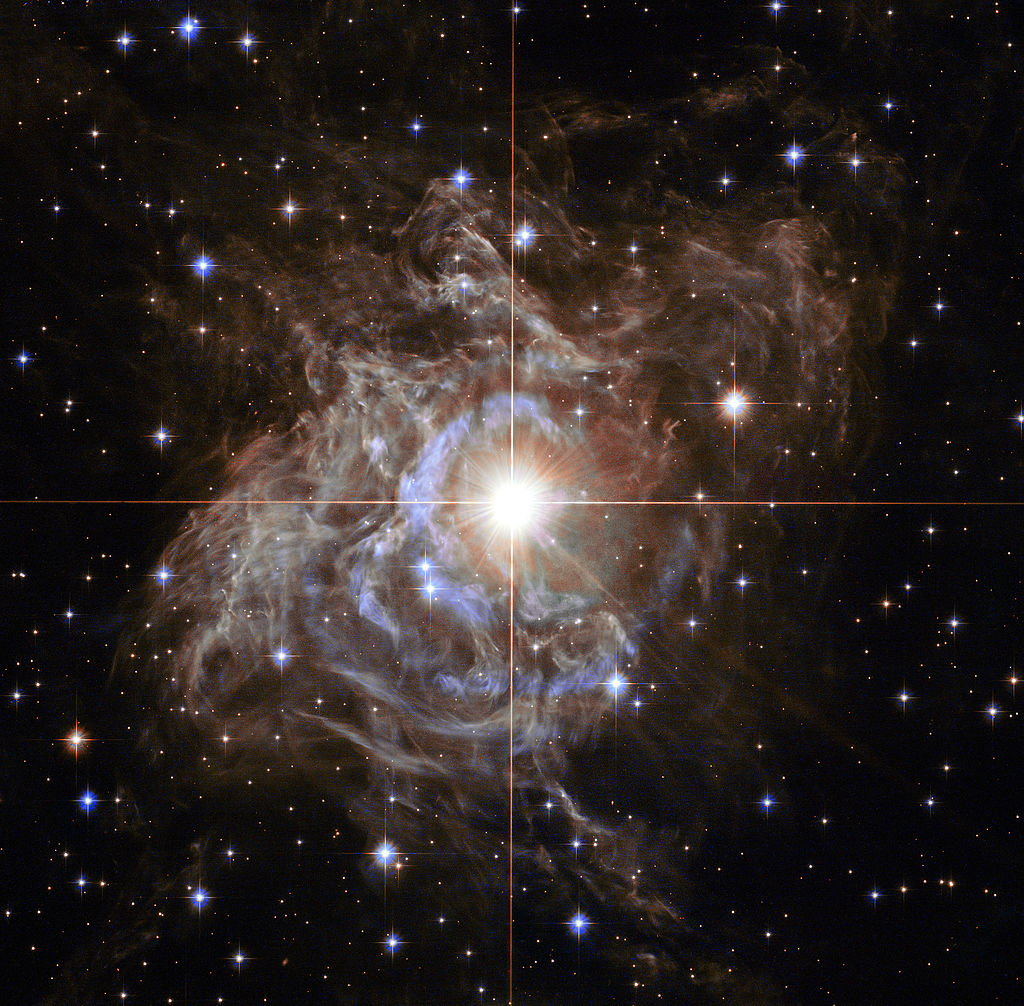
\includegraphics[height=0.9in,]{cepheids}}
\subfigure[造父变星光变曲线] {\includegraphics[height=0.9in]{cepheids_lightcurve}}
\subfigure[亮度-周期曲线] {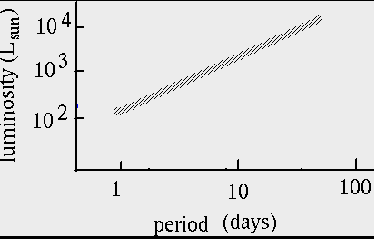
\includegraphics[height=0.9in]{cepheids_luminosity}}
\caption{造父变星}
\label{cepheids}
\end{figure}
\end{frame}
\begin{frame}\frametitle{Ia型超新星(Type Ia Supernovae)}
考虑一个白矮星和伴星的系统。回忆在统计物理中白矮星是由电子简并压而形成的星体。这个星体在不断吸收伴星的质量。如果白矮星部分的质量超过钱德拉塞卡极限$(\sim 1.4 M_{\odot})$,那么电子简并压不足以对抗引力,就会产生超新星爆发的现象。
\begin{figure}[!t]
\centering
\subfigure[超新星爆发的遗迹] {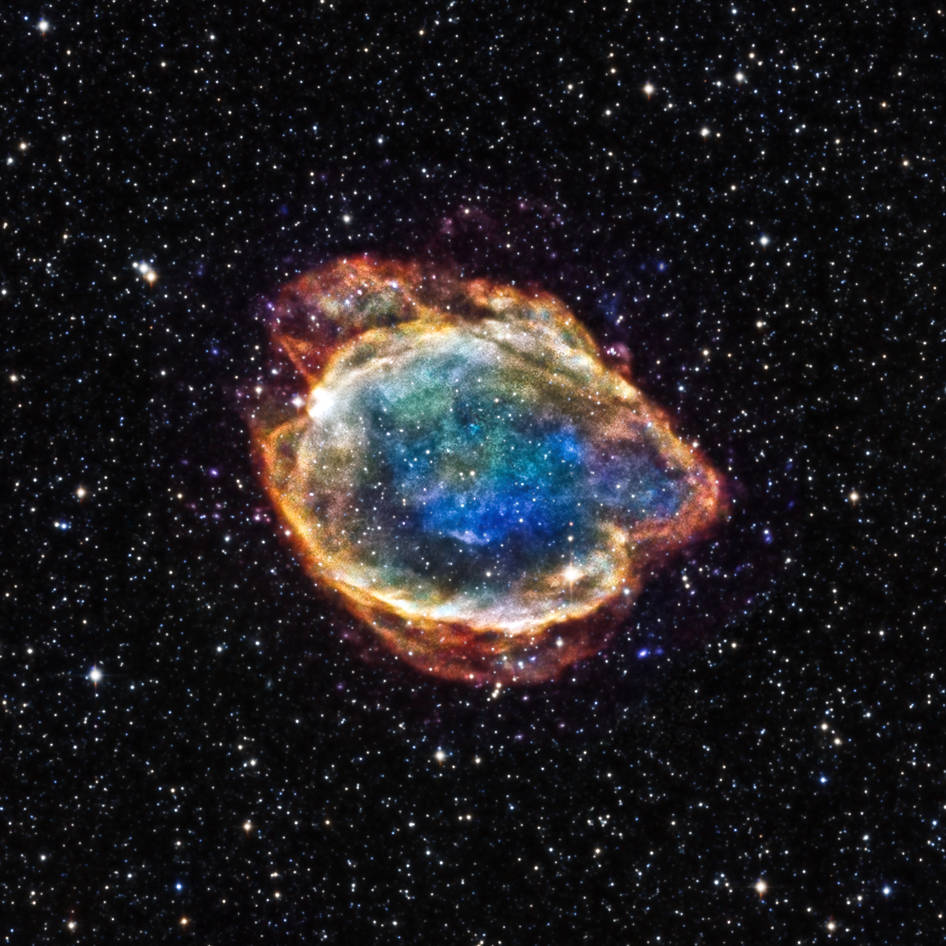
\includegraphics[height=1.2in]{G299}}
\subfigure[超新星产生的物理过程] {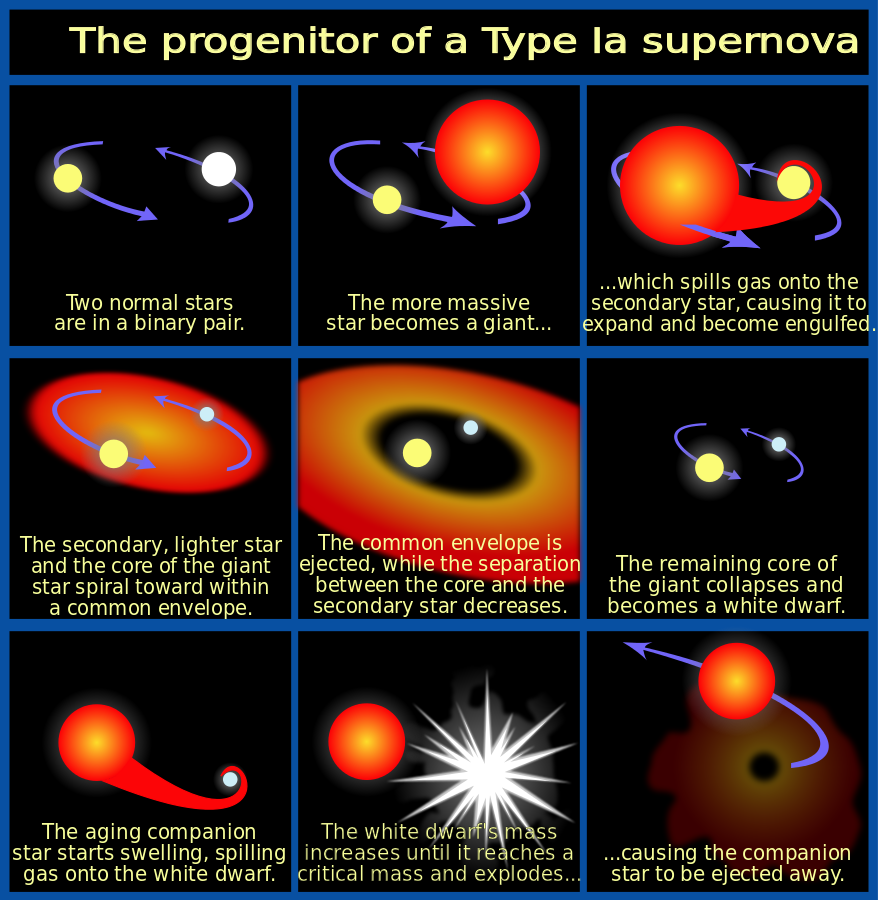
\includegraphics[height=1.2in]{Ia_supernovae}}
\caption{超新星}
\label{cepheids}
\end{figure}
\end{frame}
\begin{frame}\frametitle{引力波}
未来还有一种可能的辩认距离的方式可能是通过引力波。
\end{frame}
\begin{frame}\frametitle{视光度}
我们希望推导在FRW度规下,视光度$f$和绝对光度$L$的关系。视光度是指单位面积的接收器单位时间内所接收到的能量。显然,在平坦空间内,它和绝对光度$L$的关系为
\be 
f = \frac{L}{4\pi d^2}
\ee 
其中$d$是光源到接收器的距离。我们其实只需要考虑三项修正
\begin{itemize}
	\item FRW度规对于球面表面积的修正。
	\item 红移所引起的能量修正。
	\item 红移所引起的频率修正-单位时间内接收的光子数变少。
\end{itemize}

\end{frame}
\begin{frame}\frametitle{视光度(续)}
回忆FRW度规
\be 
ds^2 = -c^2 dt^2+a^2(t) R^2\lmbk{d\chi^2 + S_k(\chi ) \lbk{d\theta^2+\sin^2\theta d\phi^2}}
\ee 
考虑空间部分,在径向和两个角度项的小“线元”分别为$a(t)Rd\chi$,$a(t)RS_k(\chi)d\theta$,$a(t)RS_k(\chi) \sin\theta d\phi$。注意我们考虑的应该是在“今天”这个时间$t_0$,我们和那个星体所对应的物理距离,这个和光实际走过的距离是有差别的,在计算能量分配的时候,要按照这个同时的物理距离计算。于是我们取$a(t_0)=1$。

在$\chi$固定的情况下,三维球面的面积为$4\pi R^2 S_k^2(\chi)$。这就是FRW度规对于$4\pi d^2$项的修正。
\end{frame}
\begin{frame}\frametitle{光度距离(Luminosity Distance)}
根据红移的定义有
\be 
\nu_0 = \frac{\nu}{1+z}
\ee 
其中$\nu$是光发射时光的波长。所以能量也应该乘上$1/1+z$的衰减系数。

最后,我们再考虑由于红移所引起的单位时间内接收光子数变少,由上式,得知还应该乘上一个频率系数。所以最后我们得到接收到的视光度为
\be 
f = \frac{L}{4\pi R^2S_k^2(\chi)} \times \lbk{\frac{1}{1+z}}^2
\ee 
和平坦空间的式子作对比,我们定义光度距离(Luminosity Distance)
\be 
d_L = R S_k(\chi ) (1+z)
\ee 
这样视光度便可以写成
$f = \frac{L}{4\pi d_L^2}$
\end{frame}
\begin{frame}\frametitle{思考题}
我们已经发展出了第一个可以用到观测的公式
\be 
d_L = R S_k(\chi ) (1+z) = \sqrt{\frac{ f}{4\pi L}}
\ee 
这意味着在天文观测中,可以测到一个星体的$(z,f)$,知道了$f$就相当于知道了$d_L$。你能从一系列低红移的超新星曲线中拟合出哈勃常数吗?宇宙膨胀的加速度呢?上网找点数据试试?(提示:假设$k=0$,将$R\chi $使用哈勃常数和加速度泰勒展开)

最后,从你的结果可以看出,我们现在的宇宙是如何膨胀的,在加速还是在减速?这符合你的直觉吗?为什么?
\end{frame}
\end{document}
